\chapter{\uppercase{$^{227}$Ac as a Calibration Source}} \label{ch:Ac}

\section{Motivation}

In the absence of an eV-scale sterile neutrino PROSPECT should measure IBD rates that fall like one over distance from the reactor squared. 
If sterile neutrino oscillation was detected, after one year PROSPECT would measure the spectrum seen in Figure~\ref{fig:lovere1yr}, given a mass splitting of 1.78 eV$^2$, .
However, a situation could occur in which a sterile neutrino did not exist, or could not be measured with PROSPECT, and an oscillation is still measured.
This could happen if there are segment to segment volume variations throughout the detector, mimicking an oscillation signal.
Therefore, it becomes important that the product of efficiency$\times$volume for all segments is well known. 

\begin{figure}[h]
	\centering
	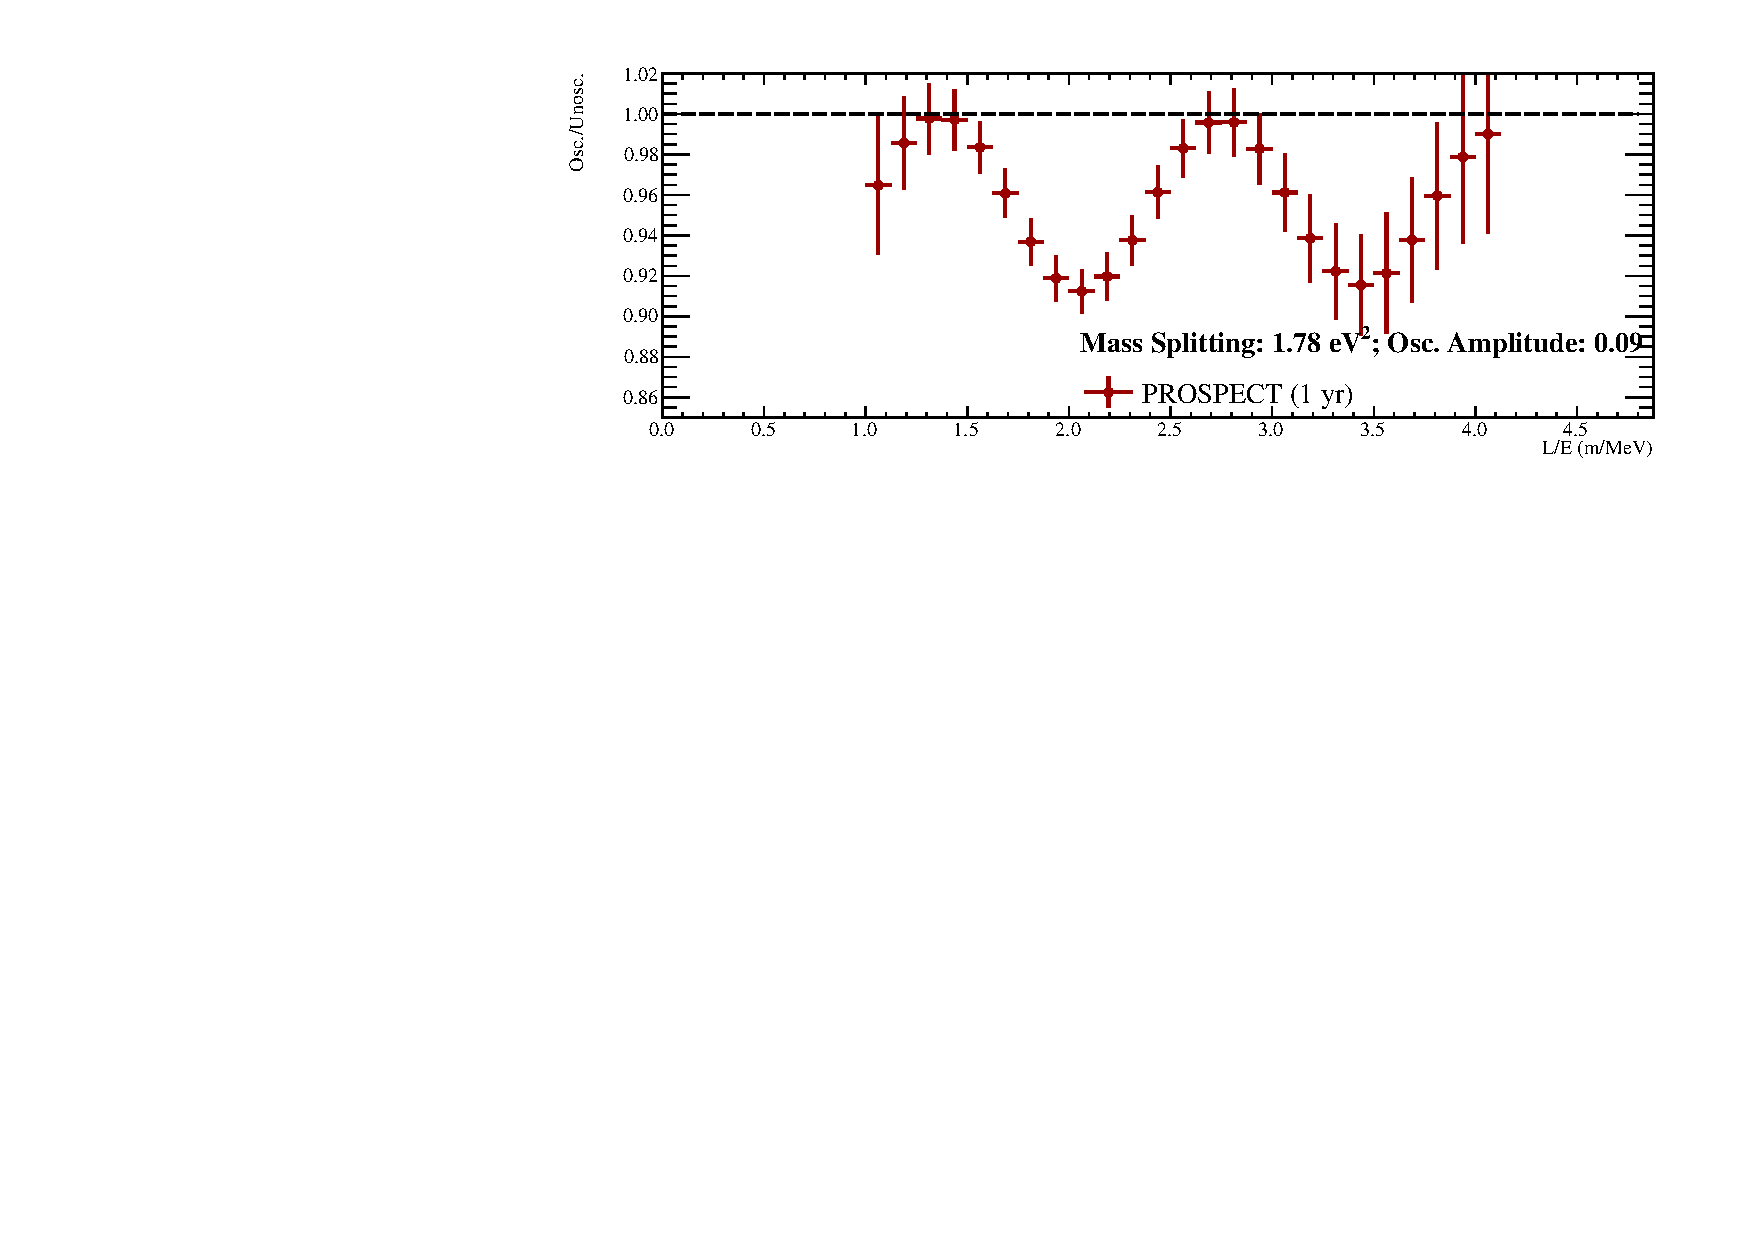
\includegraphics[width=0.7\linewidth]{tex/6-ac227-images/LoverE_1yr}
	\caption[Monte Carlo neutrino spectrum as a function of L/E]{The ratio of the oscillated to un-oscillated neutrino spectrum as a function of L/E that would be observed by PROSPECT after 1 year if a sterile neutrino signal was detected \cite{PSurukuchi:1534}.}
	\label{fig:lovere1yr}
\end{figure}


This measurement can be accomplished if an event source is uniformly distributed throughout the active volume of the detector. 
By measuring the rate of this source in each segment the relative volumes can be compared and tracked through time.
\Ac was chosen as the source and a chloride solution was prepared and dissolved in the liquid scintillator to ensure uniform distribution.

\Ac was chosen for several reasons. First, because an \AaAa coincidence occurs in its decay chain, specifically $^{219}$Rn $\rightarrow ^{215}$Po + $\alpha \rightarrow ^{211}$Pb + \Aa, as highlighted in Figure~\ref{fig:ac227chain}.
\Rn has a half-life of 3.96 $\pm$ 0.01 s and $\alpha$-decays 100\% of the time, while \Po has a half-life of 1.781 $\pm$ 0.005 ms and $\alpha$-decays  99.99977(2)\% of the time \cite{ENSDF}, so the \AaAa coincidences happen frequently and quickly.
The \Aa decay of \Po is mono-energetic at 7.39 MeV which results in a $\sim$0.78 MeV signal after quenching, well removed from nLi captures that occur around 0.5 MeV. 
In addition, there are no corresponding gammas with the \Po decay, making this a very clean and well defined signal.
The \Rn \Aa decays are not so nice, as there are four dominant alpha energies and three dominant gamma energies for these decays, as listed in Table~\ref{tab:RnPoE}, but the use of time, energy, and PSD cuts make them easy to pair with corresponding \Po decays.

\begin{figure}[hb]
	\centering
	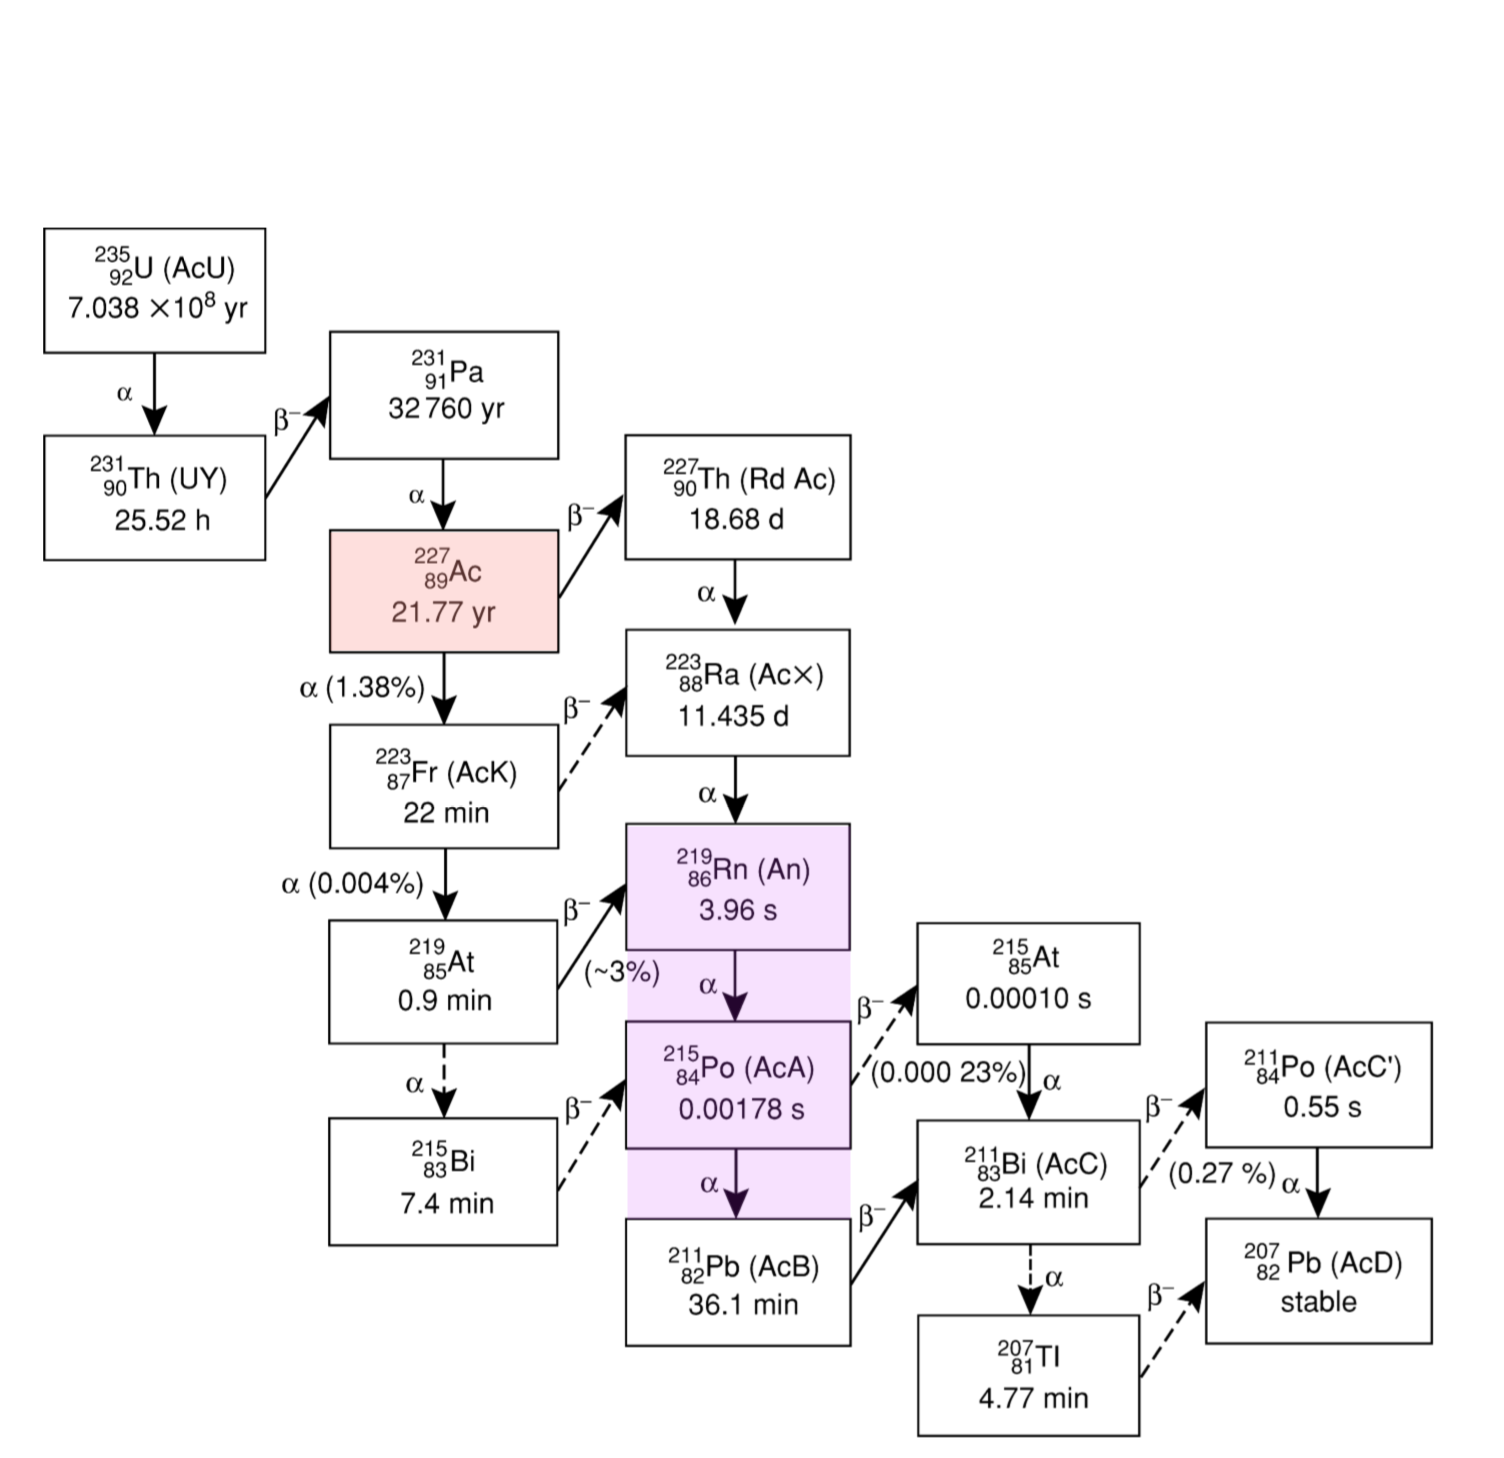
\includegraphics[width=0.6\linewidth]{tex/6-ac227-images/Ac227Chain}
	\caption[\Ac decay chain]{The full decay chain of \Ac (a daughter of $^{235}$U), in which the \AaAa coincidence of interest is highlighted \cite{Kirby2011}.}
	\label{fig:ac227chain}
\end{figure}

\begin{table}[h]
	\centering
\begin{tabular}{|c|c|c|c|c|c|}
	\hline 
	& E$_\alpha$ [keV] & I$_\alpha$ \% &  & E$_\gamma$ [keV] & I$_\gamma$ \% \\ 
	\hline 
	\Rn & 6425.0(10) & 7.5(6) &  & 271.23(1) & 10.8(6) \\ 
	%\hline 
	& 6530(2) & 0.110(10) &  & 401.81(1) & 6.6(4) \\ 
	%\hline 
	& 6552.6(10) & 12.9(6) &  & 130.60(3) & 0.13(9) \\ 
	%\hline 
	& 6819.1(3) & 79.4(10) &  &  &  \\ 
	\hline 
	\Po & 7386.1(8) & 99.999770(20) &  &  &  \\ 
	\hline 
\end{tabular} 
\caption[$\alpha$ and $\gamma$ energies of \Rn and \Po decays]{Energy and absolute intensity of dominant $\alpha$ and $\gamma$ decay radiation for \Rn and \Po. Decay energies not listed here have an intensity of $< $0.05\%.}
\label{tab:RnPoE}
\end{table}

%\begin{figure}[h]
%	\centering
%	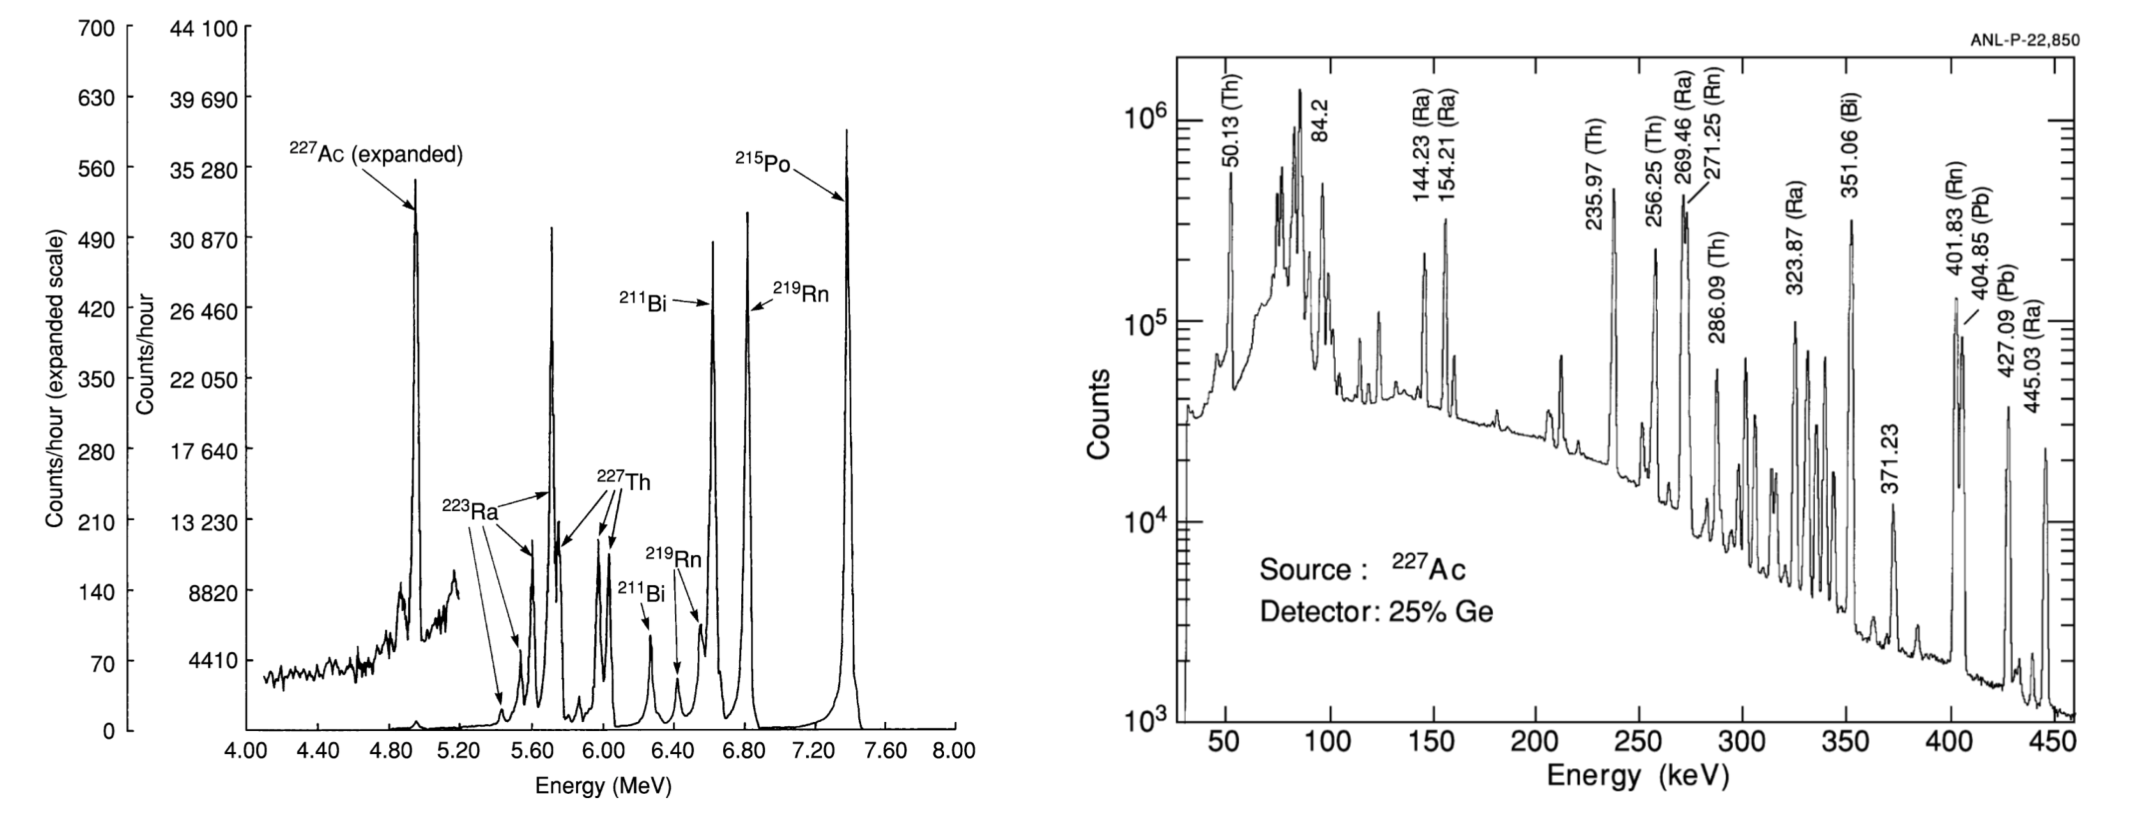
\includegraphics[width=0.95\linewidth]{tex/6-ac227-images/Actinium_agSpectrum}
%	\caption[]{\cite{Kirby2011}}
%	\label{fig:actiniumagspectrum}
%\end{figure}



\section{Material Compatibility}


\section{Event Selection in the PROSPECT AD}

\section{Detector Stability Results}

\section{Volume Variation Results}

